\chapter{Grundlagen} \label{chap:Grundlagen}
\thispagestyle{empty}
In diesem Kapitel wird zunächst eine Einführung in alle Themenbereiche gegeben. Insbesondere wird der modellprädiktive Pfadfolgeregler näher erläutert, um ein besseres Systemverständnis zu erlangen. Außerdem wird auf  Strategien für das Überprüfen von Software und Testabläufe, speziell in der Automobilindustrie, näher eingegangen und ein Einblick in aktuelle Softwareentwicklungsabläufe gegeben. 
\section{Modellprädiktive Pfadfolgeregelung} \label{sec:MPFC}
\subsection{Modellprädiktive Regelung}
Die modellprädiktive Regelung ist ein Verfahren zur Regelung von dynamischen Systemen. Dabei wird ein mathematisches Modell des Systems erstellt. Durch das messen und beobachten des Ausgangszustandes können über die Gleichung \ref{eq:mpc_schema} die zukünftigen Systemzustände $x$ und Ausgänge $y$ innerhalb des Prädiktionshorizonts $n_p$ vorhergesagt werden. Das prädizierte Systemverhalten wird dann verwendet, um ein Optimalsteuerungsproblem (engl. Optimal Control Problem, OCP) zu lösen und die optimale Eingabe zu finden, um das System in einen gewünschten Zustand zu bringen.
\begin{equation}
    \begin{split}
        x(k+1)  &= f(x(k), u(k)) \\
        y(k)    &= g(x(k), u(k))
    \end{split}
    \label{eq:mpc_schema}
\end{equation}
Der Ablauf einer modellprädiktiven Regelung wie in Abbildung \ref{fig:MPC} kann in drei Punkte unterteilt werden \cite{camacho2013model}:
\begin{enumerate}
    \item Mithilfe eines Modells wird der Ausgang eines Systems $y(k+i)$ für die nächsten $i = 1, ..., n_p$ Zeitschritte vorausgesagt. Grundlage für die Prädiktion sind die aktuellen Systemzustände und -eingänge und die zukünftigen Eingänge, welche im nächsten Schritt berechnet werden.
    \item Innerhalb des Stellhorizonts $n_c$, wobei $n_c \leq n_p$, wird die Stellgrößensequenz $u$ berechnet. Dabei wird eine Kostenfunktion, beispielsweise Gleichung \ref{eq:cost_function_mpfc}, so gewählt, dass sich ein gewünschtes Systemverhalten einstellt. Häufig wird dabei ein quadratisches Gütemaß verwendet. Ebenfalls können Beschränkungen, von z.B. den Eingangsgrößen, berücksichtigt werden. Für jeden Zeitschritt wird so das OCP gelöst.
    \item Das erste Element des Stellhorizonts wird auf das System angewendet. Stell- und Prädiktionshorizont verschieben sich um einen Zeitschritt in die Zukunft. Der Zyklus beginnt von vorn. 
\end{enumerate}
\begin{figure}
    \centering
    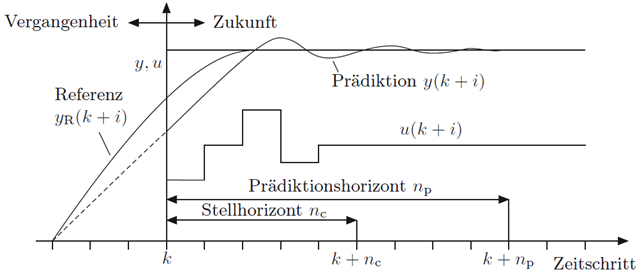
\includegraphics[width=0.8\textwidth]{figures/2_Grundlagen/MPC_Diagramm.png}
    \caption{Ablauf einer modellprädiktiven Regelung \cite{adamy2014}}
    \label{fig:MPC}
\end{figure}

\subsection{Pfadfolgeregelung}
Die Struktur der modellprädiktiven Pfadfolgeregelung, für die in diesem Praktikum eine Teststrategie implementiert werden soll, ist in Abbildung \ref{fig:MPFC_Schema} dargestellt und in \cite{ritschel2019} dokumentiert. Als Eingänge dienen der MPFC eine vorgegebene Sollgeschwindigkeit, Pfaddaten, Fahrzeugzustände, vorgegebene Beschränkungen und ein Fahrzeugmodell. Als Ausgang werden Sollbeschleunigung und Solllenkradwinkelgeschwindigkeit berechnet. Die Grundidee der Pfadfolgeregelung ist in \cite{Faulwasser2009} beschrieben. Der Regler soll einem vorgegebenen Pfad möglichst gut folgen. Im Gegensatz zu trajektorienbasierten Ansätzen ist dabei nicht vorgegeben, wann das System an welcher Stelle des Pfades sein soll. Die Regelung der Längsgeschwindigkeit ist daher zusätzlich erforderlich.
\begin{figure}
    \centering
    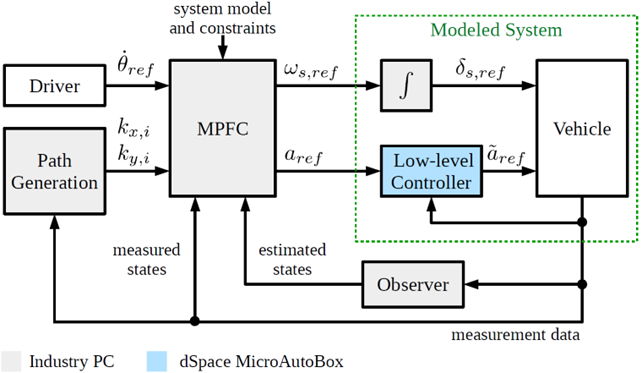
\includegraphics[width=0.8\textwidth]{figures/2_Grundlagen/MPFC_Schema.png}
    \caption{schematischer Aufbau der MPFC \cite{ritschel2019}}
    \label{fig:MPFC_Schema}
\end{figure}

\medskip \noindent Betrachtet wird das zeitkontinuierliche, nichtlineare System der Form 
\begin{align}
    \dot{x}(t)  &= f(x(t),u(t)), x(t_0)= x_0\\
    y(t)        &= h(x(t)) 
\end{align}
mit den Zuständen $x\in\mathcal{X}\subseteq\mathbb{R}^{N_x}$, Eingängen $u\in\mathcal{U}\subseteq\mathbb{R}^{N_u}$ und dem Ausgang \linebreak $y\in\mathcal{Y}\subseteq\mathbb{R}^{N_y}$. Die geometrische Kurve $\mathcal{P}:\{p(\theta)\in\mathbb{R}^{N_y}|\theta\in[\theta_0,\theta_1]\mapsto p(\theta)\}$ ist als Referenzpfad gegeben und wird durch $p(\theta)$ parametrisiert.
\begin{equation}
    p(\theta) = 
    \begin{bmatrix}
        x_{\text{ref}}(\theta) \\
        y_{\text{ref}}(\theta) \\
        \psi_{\text{ref}}(\theta)
    \end{bmatrix}    
\end{equation}
Der Pfadparameter $\theta$ gibt die Position auf dem Referenzpfad an. Dieser wird als ein virtueller Zustand von einem zusätzlichen Eingang, der Geschwindigkeit $\vartheta\in\mathcal{V}\subseteq\mathbb{R}$, beeinflusst. Dadurch ist eine Geschwindigkeitszuweisung möglich.
\begin{equation}
    \dot{\theta}(t)=\vartheta(t)
\end{equation}
\noindent Es kann nun ein Regler für das Lösen des Pfadfolgeproblems mit Geschwindigkeitszuweisung entworfen werden, der folgende Eigenschaften besitzt:
\begin{enumerate}
    \item Der Ausgang des Systems $y$ konvergiert auf den Pfad $\mathcal{P}$: $\lim \limits_{t \to \infty} \|e(t)\| = 0$ mit der Pfadabweichung $e(t) := h(x(t)) - p(\theta(t))$.
    \item Die Pfadgeschwindigkeit konvergiert auf die Referenzgeschwindigkeit: $\lim \limits_{t \to \infty} \|\dot{\theta}(t)-\dot{\theta}_{ref}(t)\| = 0$
    \item Die Zustandsbeschränkungen $\mathcal{X}$ und Eingangsgrößenbeschränkungen $\mathcal{U}$ werden eingehalten.
\end{enumerate}
\medskip
\noindent Das OCP, welches zu jedem diskreten Zeitpunkt $t_k=kT_s$ mit der Samplingzeit $T_s$ gelöst werden soll, ist folgendes:
\begin{subequations}
\begin{align}
    J(x(t_k),\theta(t_k),\bar{u}^{*}(\cdot),\bar{\vartheta}^{*}(\cdot)) = &\underset{u(\cdot), \vartheta(\cdot)}{\min} J(x(t_k), \theta(t_k), \bar{u}(\cdot), \bar{\vartheta}(\cdot)) \label{eq:minProblemA}\\
    s.t \hspace{30pt} &\dot{\bar{x}}(\tau) = f(\bar{x}(\tau), \bar{u}(\tau)), \quad \bar{x}(t_k) = x(t_k) \label{eq:minProblemB}\\
    &\dot{\bar{\theta}}(\tau) = \bar{\vartheta}(\tau), \quad \bar{\theta}(t_k) = \theta(t_k) \label{eq:minProblemC}\\
    &\bar{e}(\tau) = h(\bar{x}(\tau)) - p(\bar{\theta}(\tau)) \label{eq:minProblemD}\\
    &\bar{u}(\tau) \in \mathcal{U}, \quad \bar{x}(\tau) \in \mathcal{X} \label{eq:minProblemE}\\
    &\bar{\theta}(\tau) \in [0, \theta_{max}], \quad \bar{\vartheta}(\tau) \in \mathcal{V} \label{eq:minProblemF}\\
    &h_c(\bar{x}(\tau), \bar{u}(\tau)) \leq 0 \label{eq:minProblemG}
\end{align}
\end{subequations}
\noindent Die zu minimierende Kostenfunktion ist gegeben mit:
\begin{multline}
    J(x(t_k),\theta(t_k),\bar{u}(\cdot),\bar{\vartheta}(\cdot)) = \\ \int_{t_k}^{t_k + T_p} F(\bar{e}(\tau),\bar{x}(\tau),\bar{u}(\tau),\bar{\vartheta}(\tau))d\tau + E(\bar{e}(t_k+T_p),\bar{x}(t_k+T_p))
    \label{eq:cost_function_mpfc}
\end{multline}
\noindent Prädizierte Systemzustände und Eingänge werden mit $\bar{x}(\cdot)$ und $\bar{u}(\cdot)$, optimale Eingangsgrößen mit $\bar{u}^{*}(\cdot),\bar{\vartheta}^{*}(\cdot)$ bezeichnet. Die Systemdynamik wird durch die Gleichungen \ref{eq:minProblemB} und \ref{eq:minProblemC} repräsentiert. Die Abweichung des Systems vom Pfad geht durch Gleichung \ref{eq:minProblemD} in das Optimierungsproblem ein. Die Gleichungen \ref{eq:minProblemE} und \ref{eq:minProblemF} geben Beschränkungen für Zustände und Eingangsgrößen vor. Geschwindigkeitsabhängige Beschränkungen der Lenkaktorik werden mit Gleichung \ref{eq:minProblemG} berücksichtigt. 
\noindent Die Wegkosten $F(\cdot)$ und die Endkosten $E(\cdot)$ sind mit
\begin{align}
    F(e, x, u, \vartheta) &= \left\| \begin{matrix} e \\a_{lat}(x) \end{matrix} \right\|_Q^2 + \left\| \begin{matrix} u \\ \vartheta - \vartheta_{ref} \end{matrix} \right\|_R^2 \\
    E(e, x) &= \left\| \begin{matrix} e \\ a_{lat}(x) \end{matrix} \right\|_P^2
\end{align}
\noindent gegeben. Die Kostenfunktionen werden durch die Diagonalmatrizen $Q$, $R$ und $P$ gewichtet:
\begin{equation}
    \begin{split}
        Q &= \operatorname{diag}(q_x, q_y, q_\psi, q_a), \\
        P &= \operatorname{diag}(p_x, p_y, p_\psi, p_a), \\
        R &= \operatorname{diag}(r_a, r_\omega, r_v),
    \end{split}
\end{equation}
Die Qualität der Regelung hängt maßgeblich von einer geeigneten Wahl der Parameter in diesen Matrizen ab. Eine Methode zur Ermittlung geeigneter Parameterwerte ist in \cite{math11020465} dokumentiert. Durch eine bayes'sche Optimierung wurden Parameterwerte für eine möglichst optimale Verfolgung des Pfads und der Pfadgeschwindigkeit bei gleichzeitiger Minimierung der lateralen und longitudinalen Beschleunigungen ermittelt. Letzteres hat einen großen Einfluss auf die Wahrnehmung des Fahrkomforts \cite{BELLEM201890}.
    
\section{Szenariobasiertes Testen im Automobilbereich} \label{sec:SoftwaretestsAutomobil}
Um ein autonomes Fahrsystem zu realisieren und die Sicherheit zu gewährleisten, sind ausgiebige Test- und Verifikationsprozesse erforderlich. Dabei ist es nicht mehr ausreichend, Testdaten durch reale Testfahrten auf der Straße zu sammeln. Ein großer Anteil der Daten ist schlichtweg uninteressant, da keine kritischen Fahrsituationen auftreten. Es bietet sich daher an, in einer Datenbank die kritischen Szenarien zu erfassen und für spätere Verifikationsprozesse wieder heranzuziehen \cite{Nalic2020}.

Um Szenarien zu beschreiben und in eine Datenbank einordnen zu können, müssen diese klassifiziert werden. Eine Möglichkeit dafür ist die Einteilung nach Informationslevel (Abbildung \ref{fig:layer_model}). Die erste Ebene definiert dabei grundlegende Eigenschaften der Straße, wie etwa deren Beschaffenheit oder Grenzen. Die nächste Ebene fügt Infrastrukturobjekte wie Straßenschilder hinzu. Ebene drei enthält Informationen über temporäre Veränderungen der darunterliegenden Ebenen. Ebene vier fügt einem Szenario statische und dynamische Objekte wie andere Verkehrsteilnehmer und Manöverplanung hinzu. Zum Schluss können noch Umweltfaktoren eingefügt werden \cite{Nalic2020,Bagschik2018}.
\begin{figure}[H]
    \centering
    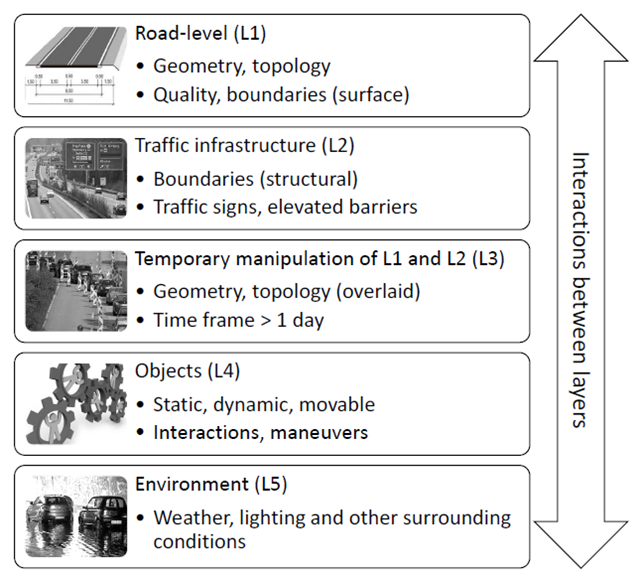
\includegraphics[width=0.5\textwidth]{figures/2_Grundlagen/layer_model.png}
    \caption{Einteilung eines Szenarios nach Informationsgehalt \cite{Bagschik2018}}
    \label{fig:layer_model}
\end{figure}

Eine weitere Klassifizierungsmöglichkeit unterscheidet die Szenarien nach dem Abstraktionsgrad (Abbildung \ref{fig:scenario_level}). Zunächst werden funktionale Szenarien beschrieben. Diese können einfach mit Worten beschrieben werden und enthalten noch keine Information über die Parameter. In einer ersten Konkretisierung  werden diese zu logischen Szenarien. Hier wurden Parameter identifiziert und Grenzen für diese festgelegt. Um ein konkretes Szenario zu erhalten, muss für jeden Parameter ein Wert ausgewählt werden. Theoretisch ermöglicht dies eine unendliche Anzahl an konkreten Szenarios, welche aus lediglich einem funktionalen Szenario erstellt werden können. Selbst bei rein simulativen Tests ist das nicht umsetzbar und muss reduziert werden \cite{Nalic2020, menzel2018scenarios}.
\begin{figure}[H]
    \centering
    
\includegraphics[width=0.7\textwidth]{figures/2_Grundlagen/scenario_level.pdf}
    \caption{Einteilung eines Szenarios nach Abstraktionsgrad \cite{menzel2018scenarios}}
    \label{fig:scenario_level}
\end{figure}

\section{Softwareentwicklungsprozesse und Unit-Tests} \label{sec:CICD}
Ein geeignetes Testmanagement erhöht die Qualität einer Software maßgeblich, indem Fehler bereits im Entwicklungsprozess entdeckt und behoben werden können. Eine Möglichkeit Testprozesse durchzuführen steckt hinter den Schlagwörtern Continuous Integration (CI) und Continuous Deployment (CD). Darunter versteht sich ein Prozess zum Entwickeln, Testen und Freigeben von Software unter Verwendung einer Versionsverwaltungssoftware, wie er in Abbildung \ref{fig:ci-cd-flow-desktop} dargestellt ist. Wenn in einem Modul einer größeren Softwareplattform Änderungen vorgenommen werden, geschieht dies in der Regel auf einer lokalen Kopie der Gesamtsoftware. Bevor diese Änderungen in das geteilte Repository für alle Entwickler übernommen werden, läuft ein automatisierter Testprozess ab (Continuous Integration). Dieser ist typischerweise in Stages unterteilt, beispielsweise build, test und merge. Dabei wird sowohl die Funktionalität eines Moduls und der Teilfunktionen (Unit-Tests), als auch das Zusammenspiel der Module untereinander (Integration-Test) überprüft. Es kann dadurch sichergestellt werden, dass die Software auch mit den Änderungen noch korrekt funktioniert. Treten in diesen Prozessschritten keine Fehler auf, werden die Änderungen übernommen und damit die Software auf den aktuellen Stand gebracht (Continuous Delivery). In einem weiteren Schritt kann die aktualisierte Software automatisiert an den Kunden ausgeliefert werden (Continuous Deployment). \cite{redhat2024}. Die Implementierung und Ausführung dieser Schritte wird häufig als \textit{Pipeline} bezeichnet \cite{Merode2023}.
\begin{figure}[H]
    \centering
    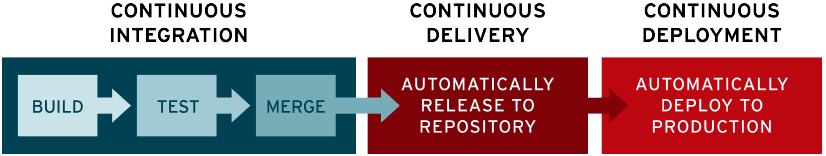
\includegraphics[width=0.7\textwidth]{figures/2_Grundlagen/ci-cd-flow-desktop.png}
    \caption{Ablauf eines CI/CD Prozesses \cite{redhat2024}}
    \label{fig:ci-cd-flow-desktop}
\end{figure}
Der kleinste Baustein in diesem Testprozess ist dabei der \textit{Unit-Test}, welcher im klassischen Sinne für die Überprüfung einer einzelnen Einheit (engl. unit) einer Software, beispielsweise einer Klasse oder einer einzelnen Funktion, zuständig ist. Dabei wird dieser Teil des Programms isoliert betrachtet und alle Abhängigkeiten durch Testcode ersetzt. Auf diese Weise kann sehr effizient der fehlerhafte Bereich des Programmcodes gefunden werden \cite{Khorikov2020}. Von der klassischen Begriffsdefinition abweichend ist die betrachtete Einheit im Rahmen dieses Berichts die gesamte Implementierung des modellprädiktiven Pfadfolgereglers. Dieser ist ein Teilmodul in dem Softwarestack für das autonome Fahren und wird durch die Bereitstellung der Simulationsumgebung isoliert. 